\section{Near-field sensor post-processing}
\label{sec:on-chip-near-field-process}

% Introduction
Near-field scan has been presented previously in \ref{sec:near-field-scan}.
Using this technique it is possible to measure maps of electric or magnetic field above a device.
While those maps already provide interesting information, to locate sources of RF noise for instance, it is interesting to post-process them in order to get voltages and currents inside the measured circuit.
In this section, two different methods are described for reconstructing the original current from a near-field magnetic measurement.
Each method requires a preliminary characterization of the probe.
Near-field scanners were extensively studied in \cite{near-field-scan, phd-monnereau}.

\subsection{Time-domain integration method}

% What is the output voltage that is measured
It is shown in \cite{near-field-scan} that the measured voltage of near-field magnetic probe is proportional to the time derivative of the measured and coupled current.
In the next part of this analysis, the sensor voltage is denoted V\textsubscript{sensor} and the original current I\textsubscript{TLP}.
The relationship between the two is expressed by Eq. \ref{eq:nfs-rel1}.
$G$ is the gain of the sensor.

\begin{equation}
V_{sensor}(t) = G.\frac{dI_{TLP}(t)}{dt}
\label{eq:nfs-rel1}
\end{equation}

% How to obtain I from V
By integrating Eq. \ref{eq:nfs-rel1}, it is possible to express I\textsubscript{TLP} as a function of the measured sensor voltage V\textsubscript{sensor}.
This is expressed in Eq. \ref{eq:nfs-rel2}.
The offset $A$ is the result of the integration.

\begin{equation}
I_{TLP}(t) = \frac{1}{G}\int V_{sensor}(t) \mathrm{d}t + A
\label{eq:nfs-rel2}
\end{equation}

% How to determine 1/G and A
Both constants $1/G$ and $A$ are determined experimentally with a preliminary calibration.
Once calculated, both factors are estimated to remain constant and can be reused in other measurements.

% Talk about calibration setup
On silicon, one of the sensors is dedicated to the calibration phase.
The setup is given in Fig. \ref{fig:calibration-sensor}.
The input of the sensor is represented by ports S1 and S2.
A square impulse of 1V amplitude generated by a 100ns wide TLP with a risetime of 8ns is injected between the two input pins.
The response V\textsubscript{sensor} is measured with a 2GHz bandwidth 10GS/s oscilloscope in differential input connected between C1 and C2.

\begin{figure}[!h]
  \centering
  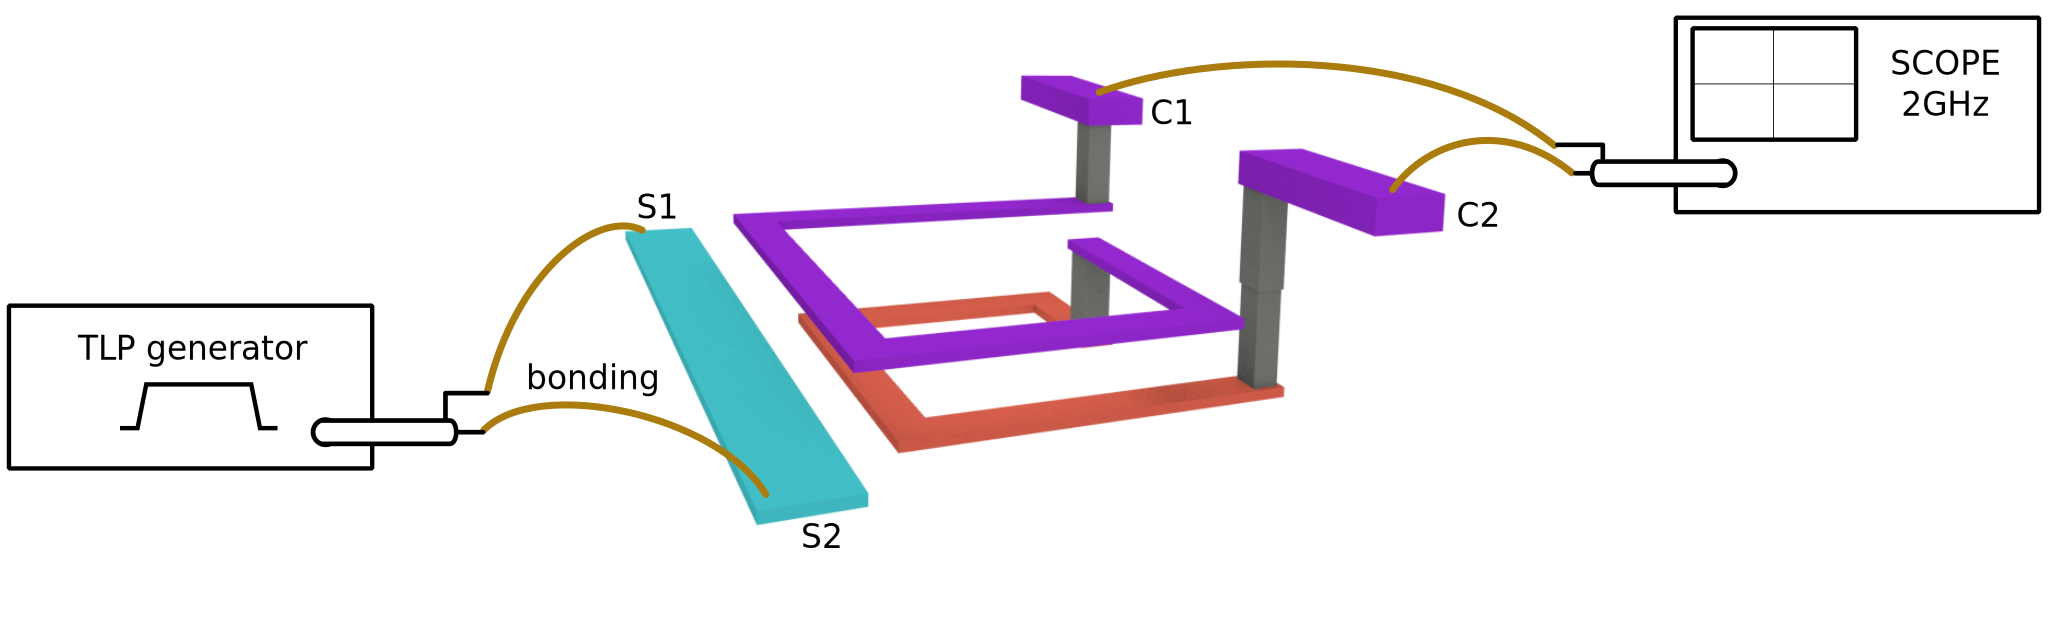
\includegraphics[width=0.9\textwidth]{src/3/figures/sensor_measurement_setup.pdf}
  \caption{Calibration sensor setup for time-domain method}
  \label{fig:calibration-sensor}
\end{figure}

% Explain the measurements
I\textsubscript{TLP} and V\textsubscript{sensor} waveforms are recorded during calibration (see Fig. \ref{fig:measurement-nfs}).
The top curve represents the input (I\textsubscript{TLP}) and the bottom curve the output (V\textsubscript{sensor}).

\begin{figure}[!h]
  \centering
  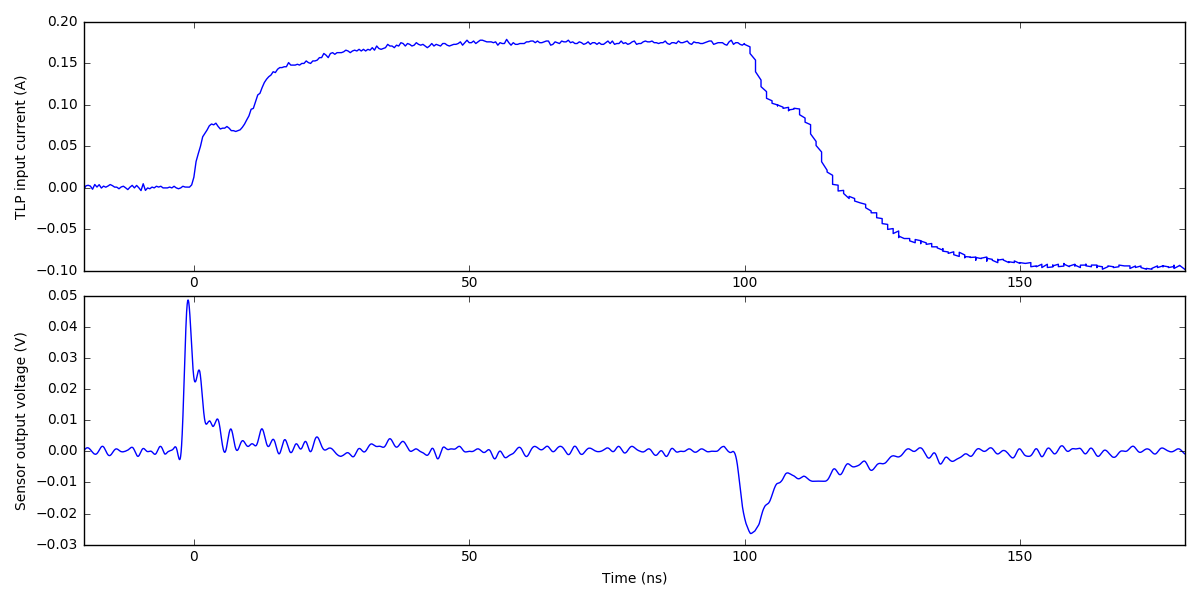
\includegraphics[width=0.9\textwidth]{src/3/figures/measured_waveform.png}
  \caption{Measured voltage waveform}
  \label{fig:measurement-nfs}
\end{figure}

% Integration method
With those measurements, $1/G$ and $A$ are determined experimentally.
Both values were estimated at $1/G = 8.10^8$ and $A = -V_{TLP}(t = 0)$ .

\begin{figure}[!h]
  \centering
  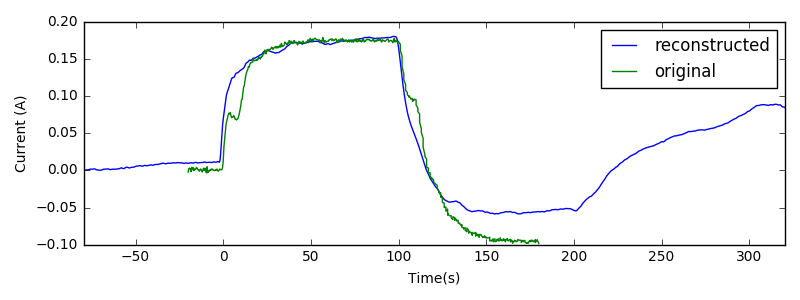
\includegraphics[width=0.9\textwidth]{src/3/figures/time_domain_vs_ref.png}
  \caption{Reference current waveform versus time-domain reconstruction}
  \label{fig:time-domain-reconstructed}
\end{figure}

% Limitations
The reconstructed curve is compared to the original in Fig. \ref{fig:time-domain-reconstructed}.
The main step of 180mA amplitude is properly reconstituted.
Differences can be seen on the rising and falling edges of the pulse.
The original curve has a first step of about 10ns wide, with an amplitude of 80mA.
This step is due to the connection cable between the load and the generator, and is fundamentally a measurement artifact.
So the difference between the two curves at 10ns and 110ns are expected.
After 110ns, a large difference is visible on the reflected part.
In most TLP analysis, the area of interest is during the pulse between 10ns and 110ns.
Therefore, those discrepancies are ignored, and the reconstitution method is considered accurate enough.

% Defaults to overcome
The time-domain method is simple to compute and produces good results.
So far, it was tested with a rectangular pulse, and in the future more cross checks should be done to ensure it works with dynamic signal such as sine waves.
The time-domain method also makes several approximations regarding the sensor's characteristics and its behavior.
It assumes that the gain of the sensor is constant for all frequencies, which is not true.
The frequency response is provided in the next section.
It should be noted that the bonding pads are also part of the calibration, but they may limit the sensor performance at high frequency.

\subsection{Frequency-domain reconstruction method}

% Intro & Characterization
The frequency-domain method post-processes the V\textsubscript{sensor} waveform using the sensor's frequency response.
The characterization is conducted with the calibration sensor, using a \gls{vna}.
The calibration setup is similar to the time-domain method.
It is given in Fig. \ref{fig:calibration-sensor-rf}.

\begin{figure}[!h]
  \centering
  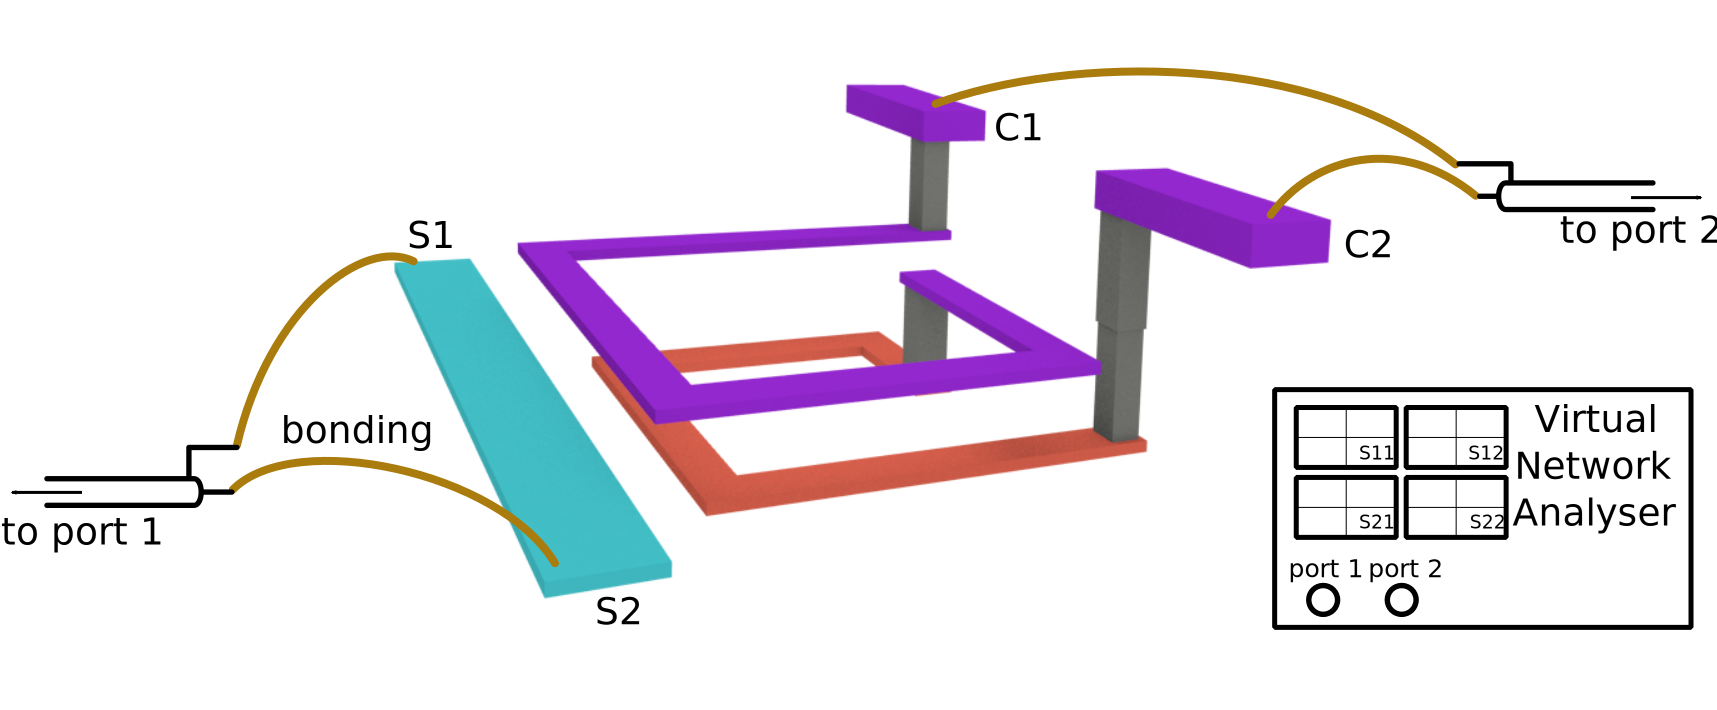
\includegraphics[width=0.9\textwidth]{src/3/figures/sensor_measurement_setup_rf.pdf}
  \caption{Calibration sensor setup for frequency-domain method}
  \label{fig:calibration-sensor-rf}
\end{figure}

% Detail characterization
The \gls{sparams} measurements of the sensor are given in Fig. \ref{fig:sensor-response}.
$S11$ is the reflected power at port 1.
$S21$ is the transmitted power between port 1 and port 2, and $S12$ is the transmitted power between port 2 to 1.
In theory, $S12$ is identical to $S21$ for symmetrical 2-port devices.
$S22$ is the reflected power from the output, which is not relevant for this study.

\begin{figure}[!h]
  \centering
  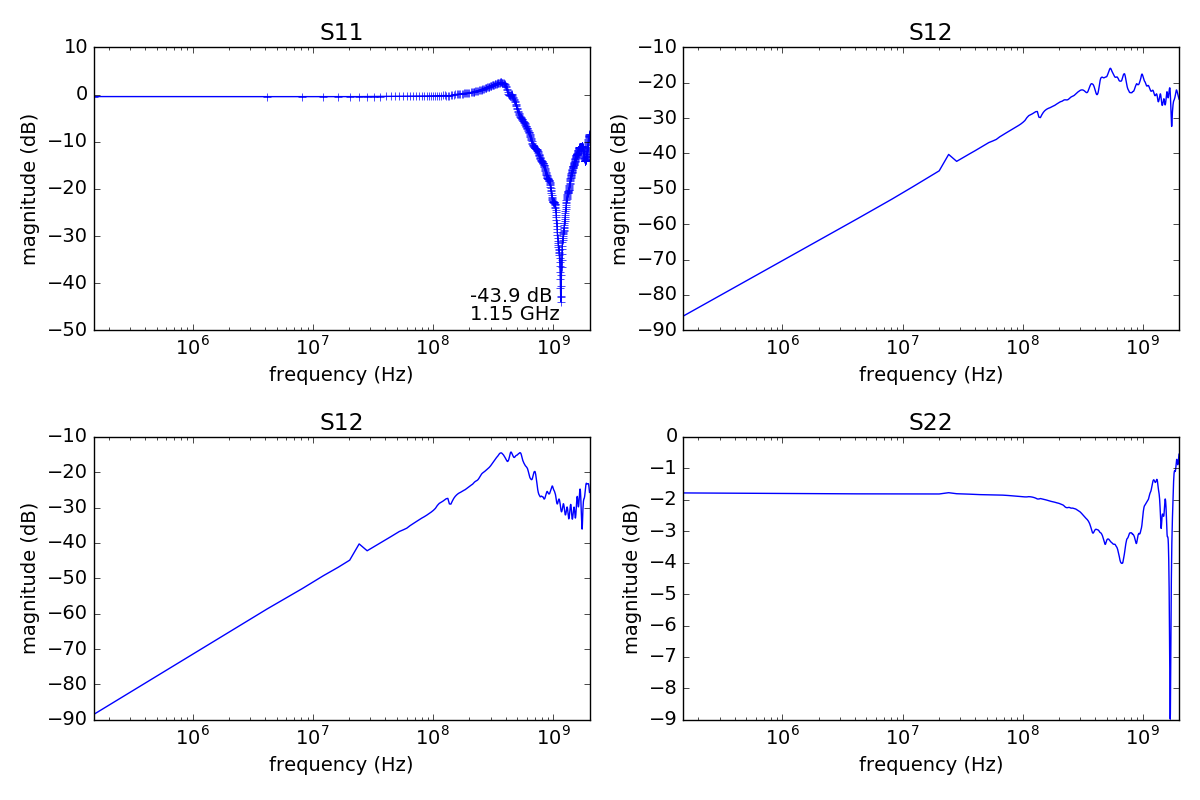
\includegraphics[width=0.9\textwidth]{src/3/figures/sensor_freq_response.png}
  \caption{Sensor frequency response}
  \label{fig:sensor-response}
\end{figure}

% Analyse the response
It was suspected previously that the sensor's response is not constant versus frequency.
The \gls{sparams} measurement confirms it, showing a sensor bandwidth of about 300MHz.
% Talk about S11
S11 shows a resonance of -43.9 dB at 1.15 GHz.
It corresponds to a frequency where insertion losses become very small.
However, this peak is not visible on the transmitted coefficient $S12$ or $S21$.
It probably means that at this frequency, a part of the input power is dissipated by the device, either by the bonding or the sensor itself.
% Talk about S21
S21 is the only scattering parameter used in the post-processing method.
It represents the transfer function between the input current and the sensed voltage.
Previously, only the magnitude measurements were displayed in Fig. \ref{fig:sensor-response}.
Another \gls{sparams} measurement has been performed, configured to obtain both magnitude and phase information (Fig. \ref{fig:s21-response-complex}).
Phase information is very helpful to improve the quality of the post-processing, as will be detailed later on.

\begin{figure}[!h]
  \centering
  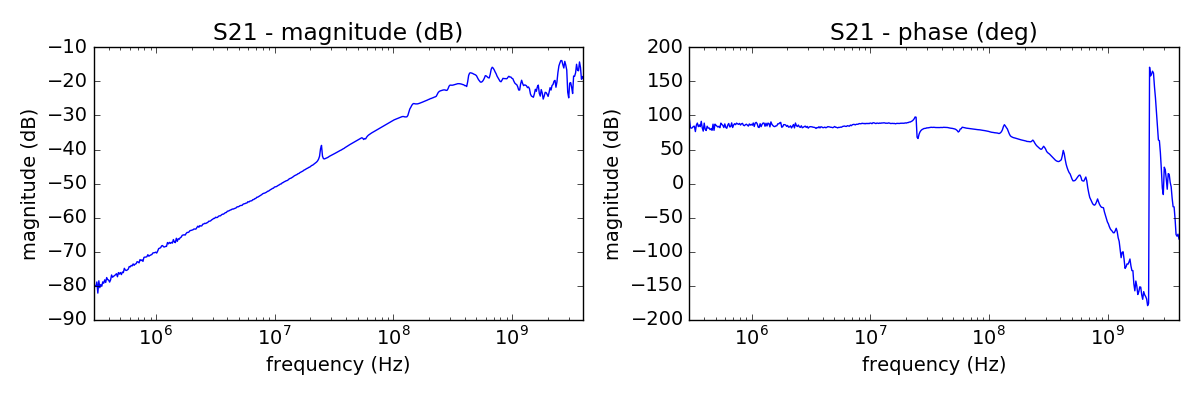
\includegraphics[width=0.9\textwidth]{src/3/figures/s21_freq_response.png}
  \caption{Sensor frequency response - complex S21 (magnitude and phase)}
  \label{fig:s21-response-complex}
\end{figure}

\begin{figure}[!h]
  \centering
  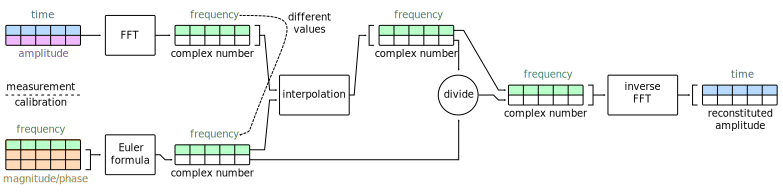
\includegraphics[width=\textwidth]{src/3/figures/frequency_post_process_flow.pdf}
  \caption{Post-processing pipeline}
  \label{fig:postprocess-nfs-pipeline}
\end{figure}

% The algorithm
The post-processing method is detailed in Fig. \ref{fig:postprocess-nfs-pipeline}.
The measurement data in the time-domain is converted to the frequency domain using \gls{fft}.
The output array associates a complex number to each frequency point.
An example is given in Table \ref{tab:complex-fft}.

\begin{table}[!h]
  \centering
  \begin{tabular}{@{}lllll@{}}
  \toprule
  frequencies (Hz)        & complex value                \\ \midrule
  1.0*10^6                & 0.33 + i0.2                  \\
  2.0*10^6                & 0.46 - i1.2                  \\
  etc.                    & etc.                         \\ \bottomrule
  \end{tabular}
  \caption{Structure for the result of (complex) FFT}
  \label{tab:complex-fft}
\end{table}

On the other hand, the S21 calibration data associates a phase and magnitude to each frequency point.
An example is given with Table \ref{tab:sparams}.
Using Euler formula (Eq. \ref{eq:to-complex}), magnitude and phase are converted to a complex number.

\begin{table}[!h]
  \centering
  \begin{tabular}{@{}lllll@{}}
  \toprule
  frequencies (Hz)          & magnitude (dB)         & phase (rad)     \\ \midrule
  1.5*10^6                  & -10                    & 1.23            \\
  2.5*10^6                  & -12                    & 0.12            \\
  etc.                      & etc.                   & etc             \\ \bottomrule
  \end{tabular}
  \caption{Structure for the S-parameter measurement}
  \label{tab:sparams}
\end{table}

\begin{equation} \label{eq:to-complex}
  S21_{complex} = 10^{\frac{magnitude}{20}} * (\cos(phase) + i*\sin(phase))
\end{equation}

% Interpolation step
After these two operations, both data are in the frequency domain.
Before moving forward in the processing, an interpolation step is required.
Indeed, the frequency points between the measurement and the calibration do not match.
For the next part of the algorithm, they need to be identical.
In this case study, a linear interpolation is employed on the measurement data to align it on the characterization.
It is possible that this kind of interpolation is not ideal.
The impact of the interpolation on the results has not been studied yet but it should be done in a future work.

% Compensation
Afterwards, the measurement data is compensated by the characterization data of the sensor.
This is done by dividing each complex value of the measurement by the complex value of the sensor.

% Inverse FFT
Finally, the inverse \gls{fft} of the compensated data is calculated to bring back the waveform into the time-domain.
The resulting waveform is compared to the original and the integration method in Fig. \ref{fig:freq-domain-reconstructed}.
Overall, the results are similar between the time-domain and frequency-domain reconstitutions.
The frequency domain seems reproduce better the rising and falling edges better.
The measurement has two short steps at the beginning and the end of the pulse, because it is performed with \gls{tdr}.
It was expected that those steps would not show up on the reconstituted waveform that should be perfectly rectangular.
There is a lot of room for improvement for each method, such as increasing the measurement frequency, and using techniques like zero-padding before performing \gls{fft} and taking dissipated power into account.
Those improvements will be evaluated and implemented as follow-up work.

\begin{figure}[!h]
  \centering
  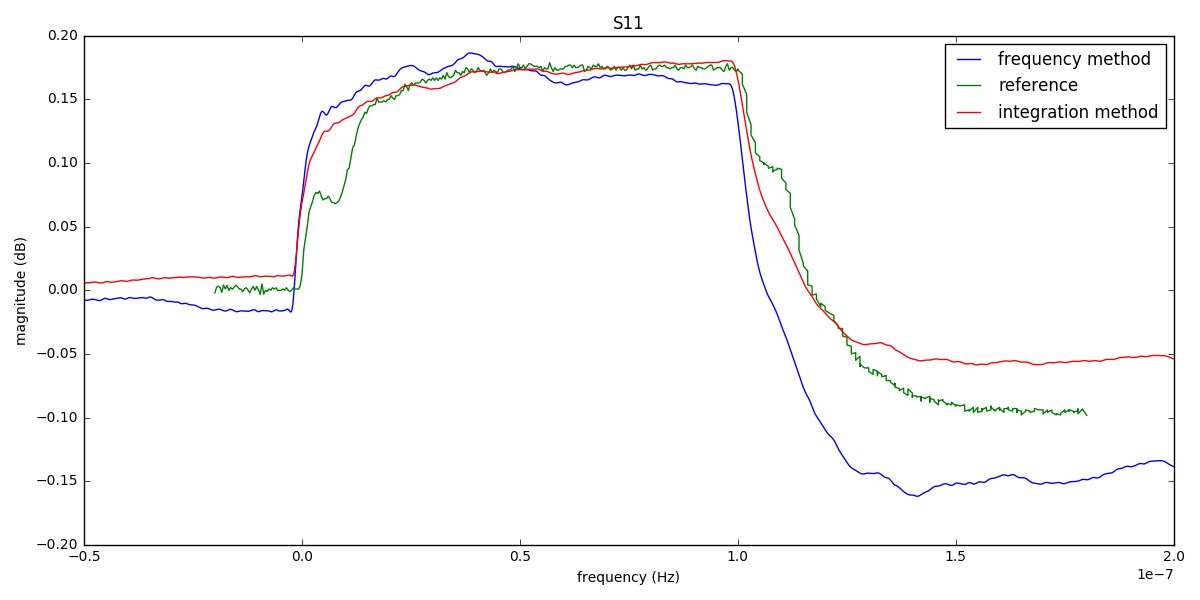
\includegraphics[width=0.9\textwidth]{src/3/figures/final_comparison_reconstructions.png}
  \caption{Reference current waveform versus frequency-domain and time-domain reconstructions}
  \label{fig:freq-domain-reconstructed}
\end{figure}

\subsection{Conclusion on near-field post-processing}

% Conclusion
In conclusion, both methods so far produce acceptable results.
The frequency method is closer to the physical properties of the device.
Ultimately, it is believed that it should behave better than the time-domain method.
It is the method chosen for processing measurement data later-on in section \ref{sec:test-vehicle-testing}

% Follow up work
As follow-up work, both techniques should be verified with sine-waves and other time varying signals.
Different integration methods and improvements to the post-processing pipeline should be tested and evaluated.

% Code repository
The two post-processing methods were implemented in Python language.
The code is freely distributed \cite{nfs-repository} as open-source software under the MIT licensing \cite{mit-licensing}.
